\documentclass[letterpaper]{article}
\usepackage{natbib,alifeconf}
\usepackage[breaklinks=true]{hyperref}
\usepackage{url}
\usepackage{graphicx}
\graphicspath{{../img/}}
\DeclareGraphicsExtensions{.pdf}

\title{EvoDraw: Evolving Interactive Animations}
\author{ Mario Garc\'ia-Valdez, Alejandra Mancilla, Georgina Aguilar, Juan-J.~Merelo$^1$\\
\mbox{}\\
Dept. of Graduate Studies at Instituto Tecnol\'ogico de Tijuana \\
$^1$Dept. of Computer Architecture and Technology and CITIC, 
University of Granada \\
{\tt mario@tectijuana.edu.mx},{\tt jmerelo@ugr.es}}

\begin{document}
\maketitle

Interactive evolutionary algorithms (IEAs) tackle the challenge of evaluating
individual's qualities (aesthetical or another), by using letting humans perform
this task. Examples of web-based IEAs are those by \cite{picbreeder} and
\cite{forms} used to evolve artistic artifacts using a generative encoding and
compositional pattern producing networks,  both presented on the web. There is
an inherent drawback in the human fatigue caused by the repeated evaluation, and
some authors have already tried to address this \citep{Frade:2010:EvoGAMES}, for
instance by simplifying the user interface by using a single button to evaluate
individuals \citep{davies2016evolving}. %how? - JJ

The present installation builds on a previous work \citep{garcia2013evospace}
but this version is directly inspired by the 1997 Galápagos interactive media
installation by \cite{galapagos} that allowed visitors to evolve 3D animated
forms. In Gal{\'a}pagos twelve computers displayed simulations of growth and
behavior of a population of abstract animated forms. Viewers participated in
this exhibit by selecting which organisms they found most aesthetically pleasing
by standing on step sensors in front of those displays. The selected organisms
survive, mate, mutate and reproduce. EvoDraw is also an IEA where through the
interaction with viewers, animations are also selected. Animations are inspired
in the Process Compendium by \cite{reas:2004}, where visual forms emerge by the
relations of multiple geometric forms and their behavior. 

In EvoDraw, viewers interact with animations by merely looking at them. Drawings
emerge from animations scripted in the Processing language, and each has an
initial setup by a list of parameters represented its chromosomes. To start the
evolutionary cycle, first, a population of animations is randomly generated and
stored in a container server called EvoSpace. Once the population is active,
client computers take animations  (their chromosome) from the server to be
presented in a monitor one at a time. After a certain amount of time, animations
are put back to the server along with information generated from the
interaction. The cycle continues by again removing another animation to be
presented to viewers. This cycle continues until there are enough interactions
to create a new generation of animations. In the previous version of this system
\citep{garcia2013evospace} viewers directly assigned a rating to each animation
via a web page; in this work, viewers only need to see the animations on
different monitors, but this time they can look at them or not, just like the
paintings inside a gallery. To assign a fitness value to each animation and thus
enabling the EA the selection of the more attractive animations, a natural user
interface device (Kinect sensor for Xbox One) it is used for facial tracking.
The sensor can track up to 6 persons at once and it provides a basic set of
information for every face: where the face is, where it is looking, among others
which are used to compute the attention received by each simulation. Each
animation is presented several times in a single generation, and those with the
best fitness are always passed to the next. To generate the new population GA
operators are applied to the population.  

\begin{figure}[!t]
\centering
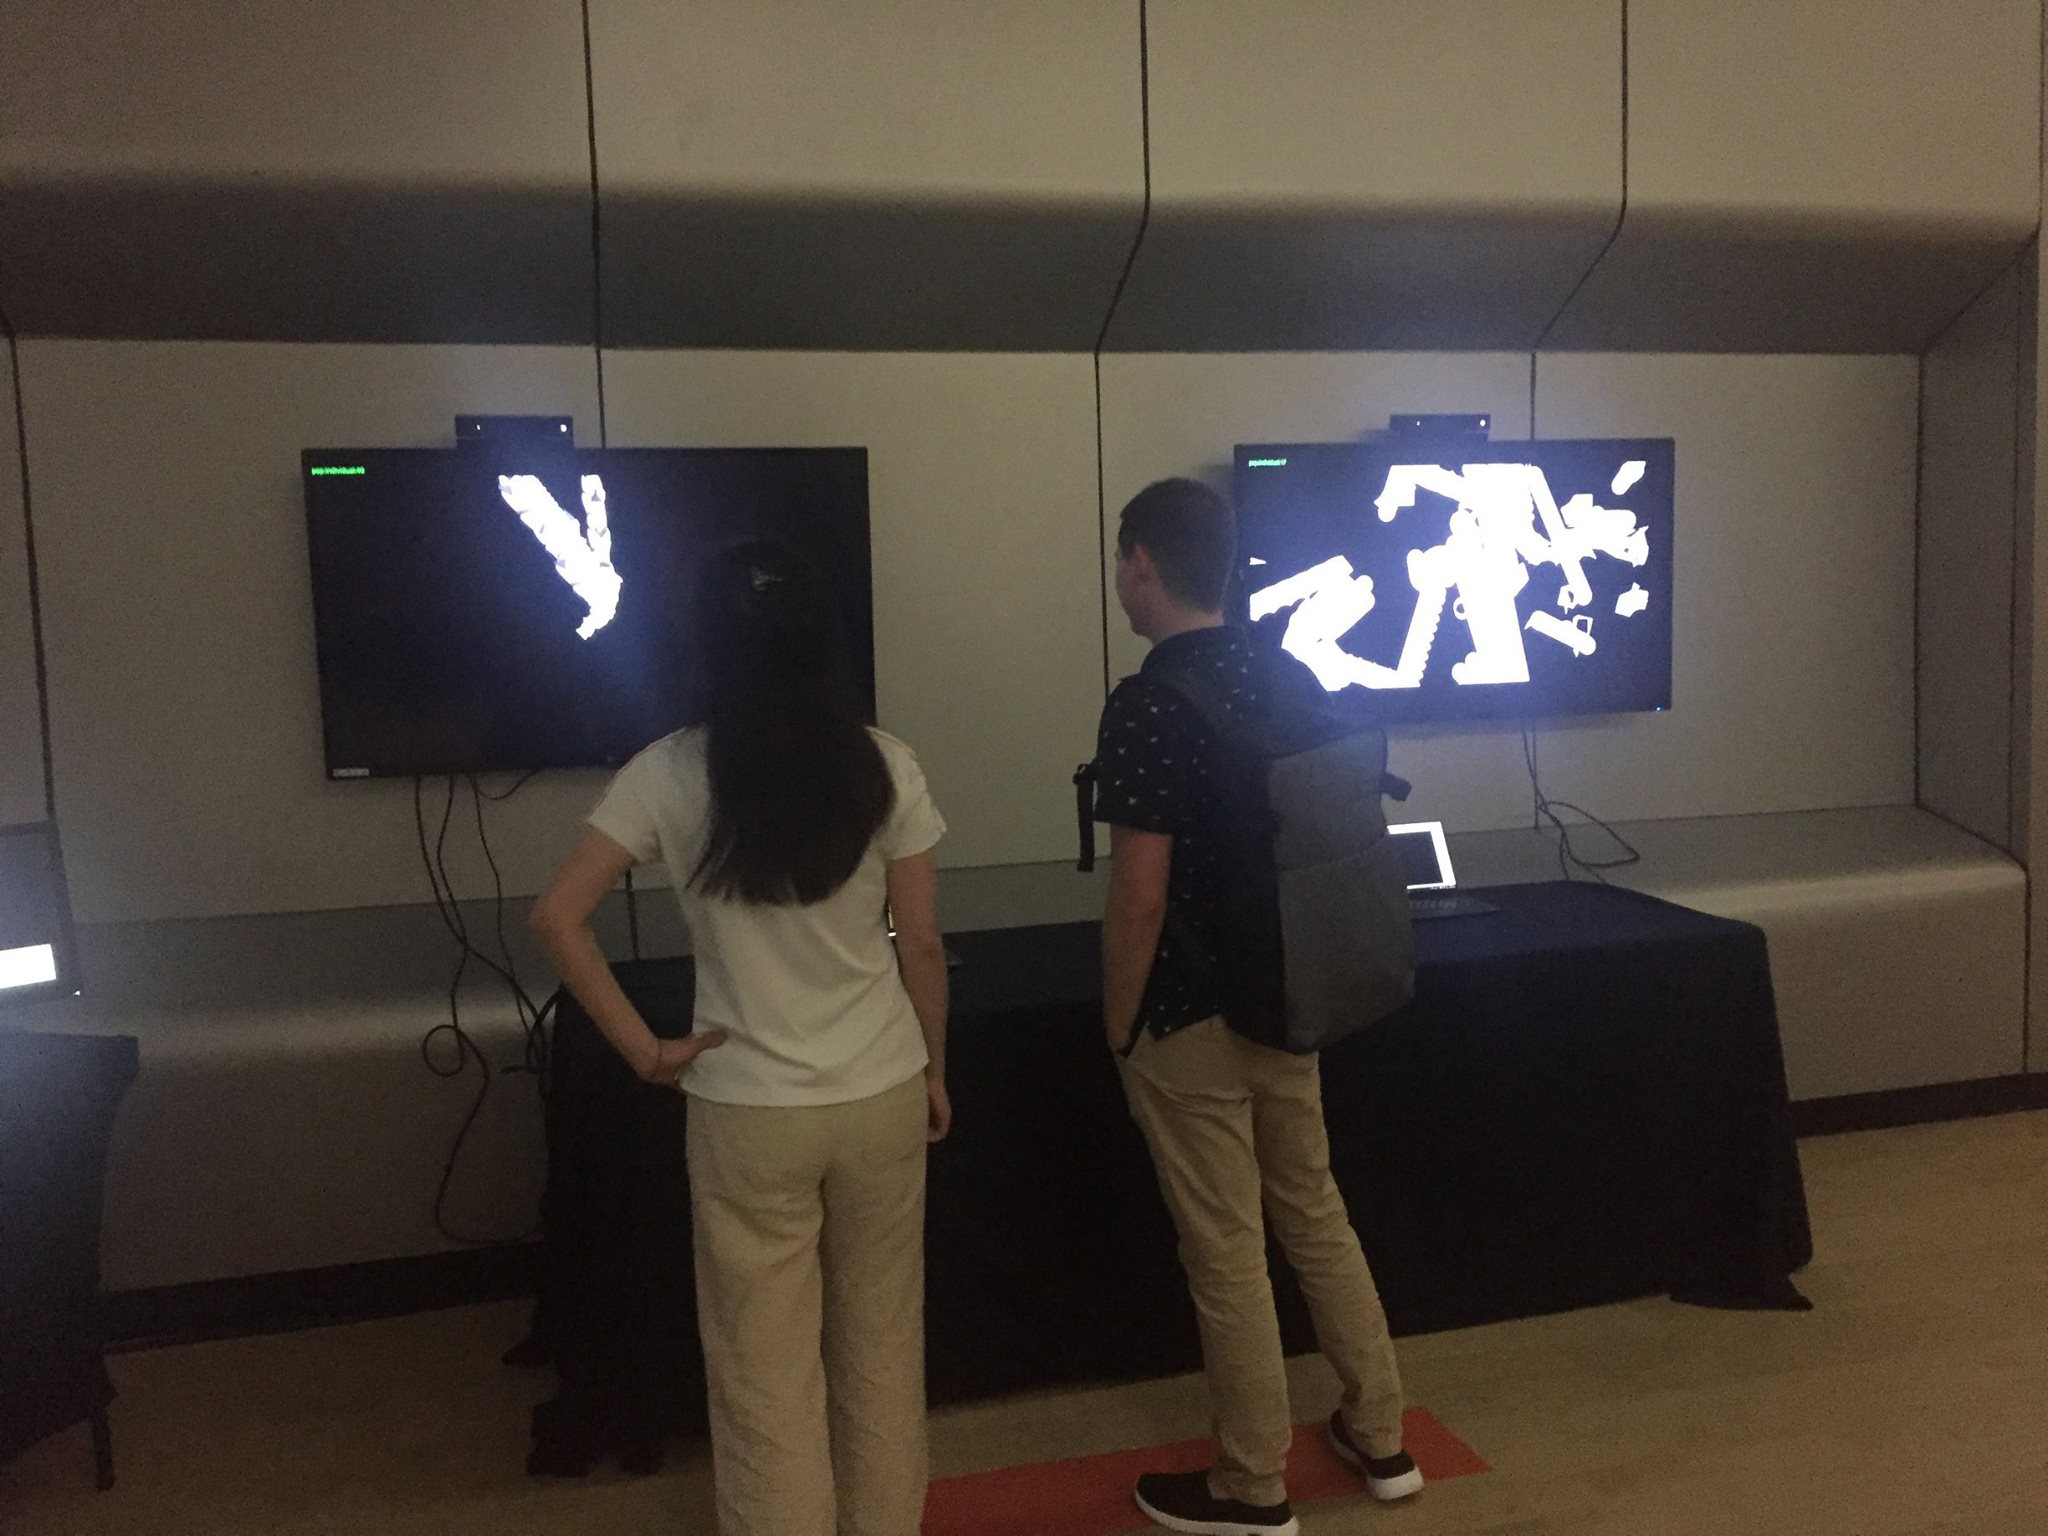
\includegraphics[width=3in]{two.jpg}
\caption{Two viewers interacting with EvoDraw in Alife XV}
\label{fig:two}
\end{figure}

\begin{figure}[!t]
\centering
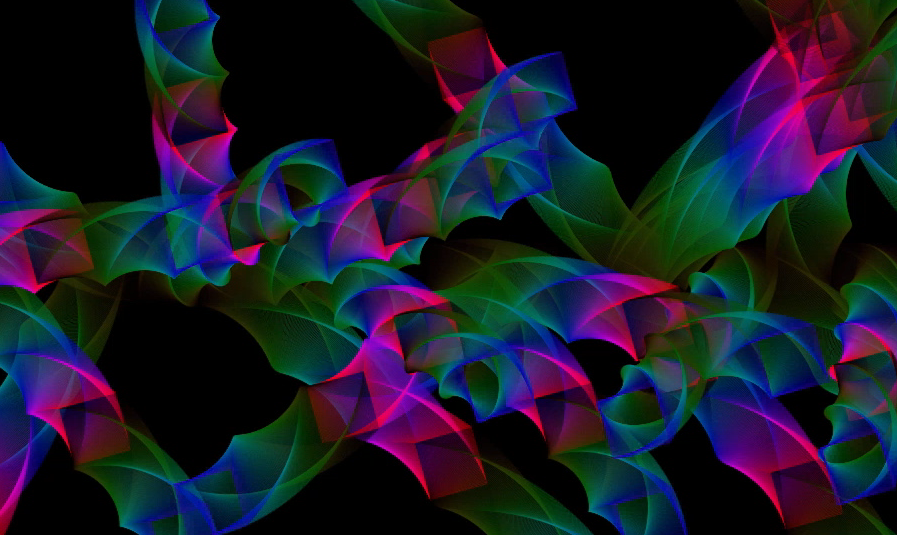
\includegraphics[width=3in]{ratings.png}
\caption{Animation generated by an IEA with explicit ratings}
\label{fig:ratings}
\end{figure}

\begin{figure}[!t]
\centering
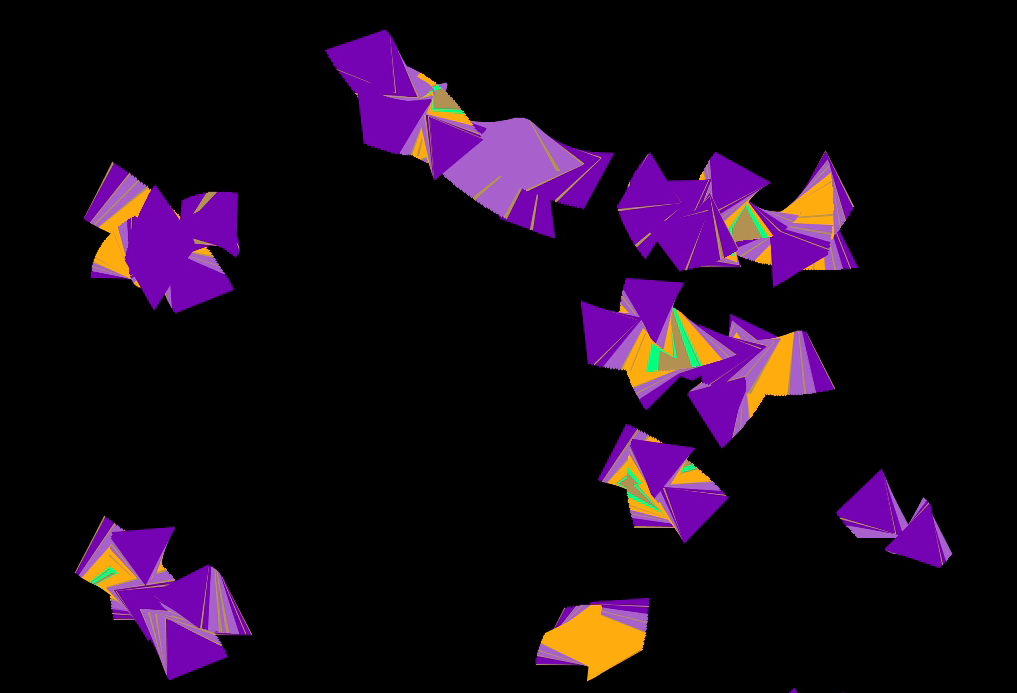
\includegraphics[width=3in]{1.png}
\caption{Randomly generated animation from Generation 1}
\label{fig:gen1}
\end{figure}

\begin{figure}[!t]
\centering
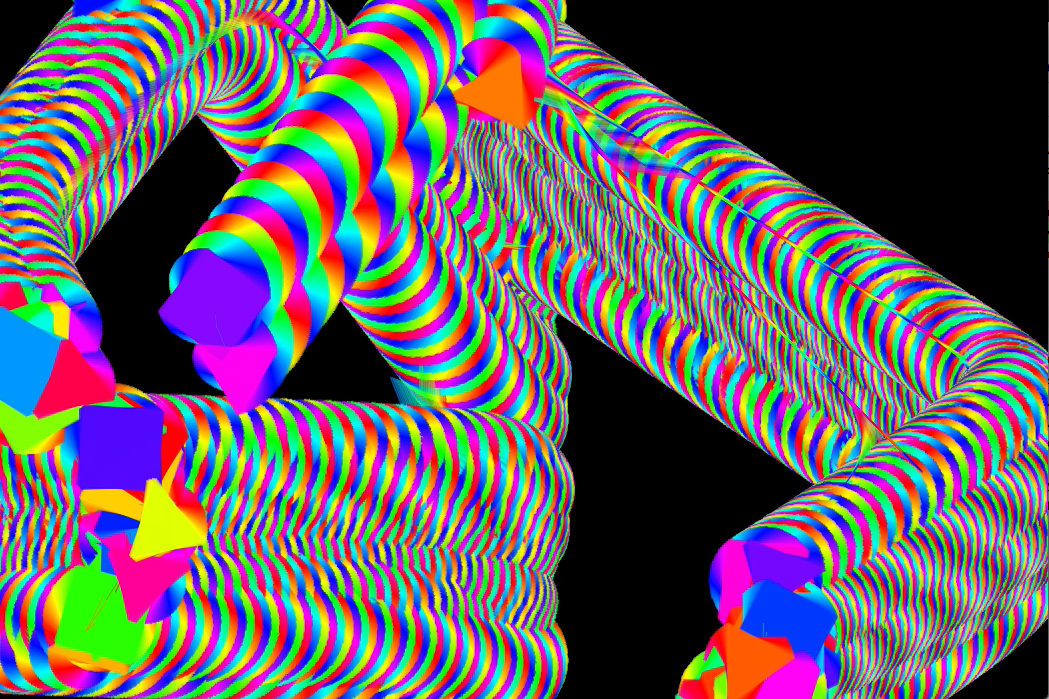
\includegraphics[width=3in]{22.png}
\caption{Animation from generation 3}
\label{fig:gen5}
\end{figure}



\begin{figure}[!t]
\centering
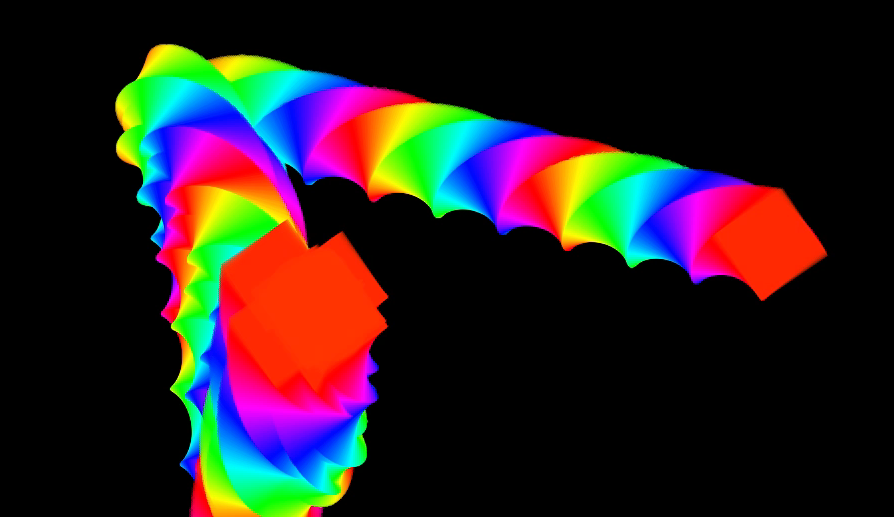
\includegraphics[width=3in]{51.png}
\caption{Animation from generation 6}
\label{fig:gen6}
\end{figure}


In this paper, we are presenting some animations generated by EvoDraw after the
execution of the algorithm on the first two days of the Alife XV conference in
Cancun, Mexico in July of 2016 (see Figure \ref{fig:two}). First, in Figure
\ref{fig:ratings} we show an example of an animation generated by another version
of EvoDraw where viewers directly assigned a rating to each animation. Then in
Figure \ref{fig:gen1} a randomly generated animation from the first generation
is shown. After some generations, (see Figures \ref{fig:5} and \ref{fig:gen6})
animations evolved to have larger figures and more bold colors.
 
One of the  goals of this work is to develop an open source framework for Web
and local IEA systems, using current web standards and libraries for mobile
devices and to explore  innovative ways in which users can be part of the IEA
algorithm. All the code of this work is available as open source from
\url{https://github.com/mariosky/evospace-js}. 


\bibliographystyle{apalike}
\bibliography{evospace-i}

\end{document}
